\chapter{Kiểm tra kiểu - Type checking}
\label{chap:typechecking}
Chương này trình bày cách giải quyết bài toán Kiểm tra kiểu thông qua các bước sau:
\begin{itemize}
\item Mở rộng ngôn ngữ assembly để lưu trữ thông tin về kiểu union.
\item Kiểm tra tính hợp lệ của việc sử dụng kiểu union trong thân chương trình.
\end{itemize}
\begin{figure}[h!]
	\centering
	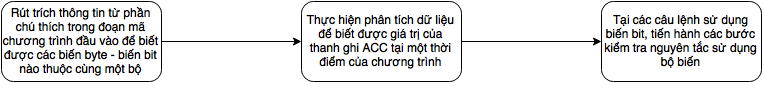
\includegraphics[width=\linewidth]{image/soDoTypeChecking}
	\caption{Sơ đồ các bước giải quyết bài toán Kiểm tra kiểu}
	\label{fig:sodotypechecking}
\end{figure}

Các phần tiếp theo của chương sẽ trình bày lần lượt các bước này.

\begin{comment}
\section{Chỉnh sửa để Boomerang chấp nhận việc sử dụng biến không phải thanh ghi}
\subsection{Cơ chế lưu trữ tên thanh ghi hiện nay của Boomerang}
Khi chuyển đổi từ mã assembly sang mã trung gian, Boomerang sẽ dùng một class con của Expr để biểu diễn thanh ghi. Cụ thể là class Location, và gọi phương thức static của class Location là Location::regOf(int num). Ta sẽ truyền vào phương thức này một con số đại diện cho thanh ghi đó. Cặp số - tên thanh ghi này được lưu vào một từ điển, để sau này khi thực hiện phân tích xong thì sẽ chuyển lại từ thanh ghi thành biến cục bộ.

Trong phần giải mã từ mã assembly sang mã trung gian, có một hàm để map giữa tên thanh ghi và con số đại diện cho nó, đó là hàm map\_sfr(string name).
\begin{lstlisting}[caption={Một số phần mã trong hàm map\_sfr},label={list:listmapsfr}]
if (name == "R0") return 0;
else if (name == "R1") return 1;
else if (name == "R2") return 2;
...
else return -1;

\end{lstlisting}

Sau khi trải qua các quá trình phân tích và đến giai đoạn in ra mã đầu ra, trình dịch ngược sẽ gọi hàm getRegName trong class FrontEnd để trả lại tên ban đầu của thanh ghi. Trong hàm getRegName sẽ lấy từ điển tên thanh ghi - số đại diện được quy định sẵn của mỗi phần giải mã cho các kiến trúc máy khác nhau, tìm tên thanh ghi tương ứng với con số đó và trả về.
\begin{lstlisting}[caption={Phần mã trong hàm getRegName},label={list:listgetregname}]
std::map<std::string, int, std::less<std::string> >::iterator it;
for (it = decoder->getRTLDict().RegMap.begin();	 it != decoder->getRTLDict().RegMap.end(); it++)
if ((*it).second == idx) 
return (*it).first.c_str();
return NULL;a
\end{lstlisting}


Như vậy, có thể thấy với các tên biến không được quy định trước, hàm map\_sfr sẽ trả về giá trị -1, và vì giá trị -1 sẽ không có trong từ điển của phần giải mã, nên hàm getRegName sẽ trả về NULL, dẫn đến trình dịch ngược sẽ bị lỗi runtime và dừng ngay lập tức.\\

%lấy mã Boomerang ban đầu về, hiện kết quả khi sử dụng biến đầu vào

Vì số lượng tên biến là rất nhiều, nên ta không thể sử dụng phương pháp thêm mới các tên biến vào từ điển được quy định sẵn được, mà phải có cách để trình dịch ngược linh động hơn, chấp nhận bất kỳ các tên nào được sử dụng trong mã assembly. Giải pháp đưa ra là ngoài việc sử dụng từ điển thanh ghi được quy định sẵn, ta sẽ lập thêm một bảng tên biến, thành phần bao gồm các cặp tên biến - số đại diện. Trong giai đoạn giải mã, khi hàm map\_sfr được gọi, nếu tên truyền vào nằm trong các thanh ghi đã quy định sẵn, thay vì trả về giá trị -1 thì ta sẽ tạo ra một giá trị random và đưa chúng vào bảng tên biến ở trên. Ngoài ra, còn có một đoạn mã kiểm tra biến được sử dụng đã được khai báo bằng câu lệnh \#DEFINE chưa (ngoại trừ một số biến đặc biệt được tự sinh). \\
\begin{lstlisting}[caption={Phần mã mới được bổ sung trong hàm map\_sfr},label={list:listmapsfrnew},language=c++]
bool isDefined = false;
map<char*, AssemblyArgument*>::iterator it;
for (it = replacement.begin(); it!=replacement.end(); it++){
if(strcmp((*it).first, name.c_str()) == 0 ){
isDefined = true;
break;
}
}
if (isDefined || name.find("specbits") != string::npos ){
if (symbolTable->find(name) == symbolTable->end()){
bool existed = false;
int num;
do{
num = std::rand()%200+31;
map<string, int>::iterator it;
for (it = symbolTable->begin(); it!=symbolTable->end(); it++){
bool cond1 = (*it).second == num;
bool cond2 = (byteVar != -1 && byteVar>=num);
bool cond3 = (bit != -1 && bit>=num);
if (cond1 || cond2 || cond3){
existed = true;
continue;
} else {
existed = false;
}
}
} while (existed); 
(*symbolTable)[name] = num;
if (name.find("specbits") != string::npos){
std::cout<<"Name: "<<name<<", "<<num<<endl;
}
return num;
} else {
return symbolTable->find(name)->second;
}
}
else {
std::cout<<"ERROR: "<<name<<" HAS NOT BEEN DEFINED YET"<<endl;
exit(1);
}
\end{lstlisting}
Tương ứng với sự thay đổi ở hàm map\_sfr,  ở hàm getRegName, ngoài việc dò trong từ điển quy định trước, ta sẽ thêm một đoạn mã để dò trong bảng tên biến. 
\begin{lstlisting}[caption={Phần mã mới được bổ sung trong hàm getRegName},label={list:listgetregnamenew},language=c++]
std::map<string,int>::iterator symIt;
for (symIt = decoder->getSymbolTable().begin(); symIt != decoder->getSymbolTable().end(); symIt++){
	if ((*symIt).second == idx){
		return (*symIt).first.c_str();
	}
}
\end{lstlisting}
Như vậy, vấn đề giữ nguyên tên biến được giải quyết mà không ảnh hưởng nhiều tới trình dịch ngược.
%đoạn mã đầu vào assembly và mã đầu ra giữ nguyên được tên biến
\end{comment}
\section{Mở rộng ngôn ngữ assembly}
Để kiểm tra được tính hợp lệ khi sử dụng kiểu union trong đoạn mã đầu vào, trình dịch ngược cần phải được cung cấp thông tin về các kiểu union thông qua một phương thức nào đó. Có hai hướng để giải quyết vấn đề này là:
\begin{itemize}
	\item Đưa ra một cấu trúc khai báo mới cho ngôn ngữ assembly. Cấu trúc khai báo này có thể tương tự như khai báo union ở ngôn ngữ cấp cao. Tuy nhiên, cách làm này sẽ làm cho đoạn mã assembly không thể compile được vì các assembler không chấp nhận cấu trúc mới thêm vào đó.
	\item Cho phép người lập trình đưa các thông tin về kiểu union vào trong phần chú thích theo một mẫu quy định từ trước. Với giải pháp này, đoạn mã không bị ảnh hưởng vì chú thích là một thành phần đã có sẵn trong ngôn ngữ assembly, và khi compile thì các assembler sẽ bỏ qua phần chú thích.
\end{itemize}
Như vậy, giải pháp thứ hai là tối ưu hơn và sẽ được áp dụng trong luận văn này. Mẫu chú thích được viết cho 8051 được thể hiện ở đoạn mã \ref{list:listdeclarevar}
\begin{lstlisting}[caption={Mẫu khai báo bộ biến},label={list:listdeclarevar}]
;BEGIN DEFINE
;DEFINE BYTE
[byte var declare]
;DEFINE BITS
[eight bit var declares]
;END DEFINE
\end{lstlisting}
Tuy nhiên, cũng giống như assembler, các trình dịch ngược hầu như sẽ bỏ qua phần chú thích khi đọc đoạn mã đầu vào, và để cho chúng có thể rút trích được thông tin từ phần chú thích thì phải thực hiện một số chỉnh sửa trong giai đoạn lexer và parser, cụ thể là:
\begin{itemize}
	\item Chỉnh sửa lexer để nhận biết các token là những chú thích đặc biệt. Như trong ví dụ \ref{list:listdeclarevar}, các chú thích ";BEGIN DEFINE", ";DEFINE BYTE", ";DEFINE BITS" không thể được đọc vào như là token COMMENT bình thường, mà phải có những token riêng biệt cho chúng để phục vụ giai đoạn parser sau đó. Đoạn mã \ref{list:8051lexer} được viết để chạy trên thư viện flex++ thể hiện điều đó. Có thể thấy, khi bắt được một chú thích, thay vì trả về token COMMENT như trước đó, phần lexer mới này sẽ kiểm tra nội dung chú thích, nếu trùng với các chú thích đặc biệt thì sẽ trả về token tương ứng. 
\end{itemize}
\begin{changemargin}{0cm}{0cm} 
	\begin{lstlisting}[caption={Phần lexer được chỉnh sửa để nhận biết các chú thích đặc biệt},label={list:8051lexer}]
	(\;.*)  { 
		string beginDefine = ";BEGIN DEFINE";
		string endDefine = ";END DEFINE";
		string defineByte = ";DEFINE BYTE";
		string defineBits = ";DEFINE BITS";
		string val = strdup(yytext);
		if (beginDefine == val)
			return BEGINDEFINE;
		else if (endDefine == val)
			return ENDDEFINE;
		else if (defineByte == val)
			return DEFINEBYTE;
		else if (defineBits == val)
			return DEFINEBITS;
		else return COMMENT;
		}
	\end{lstlisting}

\end{changemargin} 
\begin{itemize}
	\item Chỉnh sửa parser để nhận vào cấu trúc khai báo union. Tiếp tục với ví dụ mẫu khai báo \ref{list:listdeclarevar}, nếu phần parser chỉ đọc các câu lệnh khai báo biến bình thường, thì không thể xác định được các union mà người dùng khai báo trước. Như vậy, cần chỉnh sửa parser để bắt được những mẫu khai báo đặc biệt. Phần parser viết bằng thư viện bison++ cho mẫu khai báo \ref{list:listdeclarevar} được trình bày ở đoạn mã \ref{list:8051parser}. Trước khi chỉnh sửa, phần parser này chỉ có luật define, đọc vào từng câu lệnh khai báo độc lập. Sau khi được chỉnh sửa lại, luật definebit có độ ưu tiên cao hơn sẽ đọc vào cấu trúc khai báo union gồm nhiều câu lệnh khai báo khác nhau.
\end{itemize}
\begin{changemargin}{0cm}{0cm} 
	\begin{lstlisting}[caption={Đoạn mã parser nhận biết các mẫu khai báo union},label={list:8051parser}]
	definebit: BEGINDEFINE END_LINE DEFINEBYTE END_LINE 
					define DEFINEBITS END_LINE defineeachbit{8} 
					ENDDEFINE END_LINE;
	defineeachbit: DEFINE ID bit END_LINE;
	define:	DEFINE ID expressions END_LINE;
	\end{lstlisting}
\end{changemargin} 
\begin{itemize}
	\item Chỉnh sửa các hành động sau khi parser nhận biết được những cấu trúc khai báo union. Sau khi parser đã bắt được các mẫu khai báo union, cần lập trình để lưu trữ thông tin về các union đó vào dữ liệu của chương trình. Cấu trúc được dùng để lưu trữ thông tin về union này là UnionDefine, được trình bày ở đoạn mã \ref{list:listuniondefine}, trong đó, byteVar để lưu trữ tên của union đó, còn bitVar chứa các thành phần bit thuộc union và số thứ tự của bit mà thành phần đó truy xuất. Đoạn mã \ref{list:8051parser2} thể hiện phần code đưa các khai báo union từ mã đầu vào thành các thực thể UnionDefine tương ứng.
\end{itemize}
\begin{changemargin}{0cm}{0cm} 
	\begin{lstlisting}[caption={Cấu trúc dữ liệu để lưu trữ một union},label={list:listuniondefine},language=c++]
	class UnionDefine{
		public:
			char* byteVar;
			map<int, char*>* bitVar;
	};
	\end{lstlisting}
	\begin{lstlisting}[caption={Đoạn mã parser bao gồm các hành động sau khi nhận biết được union},label={list:8051parser2}]
	definebit: BEGINDEFINE END_LINE DEFINEBYTE END_LINE 
					define DEFINEBITS END_LINE defineeachbit{8} 
					ENDDEFINE END_LINE
	{
		UnionDefine* ut = new UnionDefine();
		$5 -> expList -> pop_back();
		ut->byteVar = $5 -> expList -> back() -> 
		argList.back()->value.c;
		ut->bitVar = bitVar;
		unionDefine1 -> push_back(ut);
		bitVar = new map<char*, int>();
	};
	defineeachbit: DEFINE ID bit END_LINE {
		std::string temp($3->value.c);
		char c =  temp.at(temp.size()-1);
		int num = c - '0';
		(*bitVar)[$2] = num;
	};
	define: DEFINE ID expressions END_LINE 
	{ 
		AssemblyLine* line = new AssemblyLine();
		line -> expList = new list<AssemblyExpression*>();
		line->kind = INSTRUCTION;
		line->name = "DEFINE";
		AssemblyExpression* expr1 = new AssemblyExpression();
		expr1 -> kind = UNARY;
		Arg a;
		a.c=$2;
		expr1 -> argList.push_back(new AssemblyArgument(6, a));
		line -> expList->push_back(expr1);
		line->expList ->push_back(expr);//*/
		expr = new AssemblyExpression();
		$$=line;
	};
	\end{lstlisting}
\end{changemargin} 
	
Như vậy, sau khi thực hiện các chỉnh sửa trên, trình dịch ngược đã có thể đọc vào các thông tin về union được người dùng cung cấp ở phần chú thích của đoạn mã đầu vào, đồng thời lưu trữ thông tin đó vào cấu trúc dữ liệu UnionDefine. Tuy đã xác định được những union nào được khai báo trong mã đầu vào, nhưng cần phải có một bước để kiểm tra những union đó có được sử dụng hợp lý hay không.
\section{Kiểm tra tính hợp lệ của việc sử dụng kiểu union}
Như đã trình bày ở phần \ref{sec:challenge}, ngôn ngữ assembly không cho phép thao tác trực tiếp trên các vùng nhớ, mà phải thông qua một thanh ghi trung gian và việc sử dụng một thành phần y thuộc union x chỉ hợp lệ khi mà thanh ghi trung gian đang mang kiểu union x đó. Như vậy, quá trình kiểm tra kiểu union sẽ gồm 2 bước:
\begin{itemize}
	\item Xác định kiểu của thanh ghi trung gian tại mỗi điểm của chương trình.
	\item Kiểm tra việc truy xuất thành phần của union có hợp lý hay không.
\end{itemize}
\subsection{Xác định giá trị kiểu của thanh ghi \textit{ACC} tại mỗi điểm của chương trình}
Để kiểm tra được nguyên tắc sử dụng bộ biến, trước hết, ta phải biết được tại mỗi thời điểm của chương trình, thanh ghi \textit{ACC} đang mang giá trị gì. Có hai phương pháp phân tích được áp dụng trong giải pháp này, đó là Reaching definitions kết hợp phần mở rộng và Type propagation.
\subsubsection{Phân tích Reaching definitions kết hợp phần mở rộng}
Mục đích của phân tích Reaching definitions là biết được ở một thời điểm của chương trình, các câu lệnh khai báo nào đang còn hiệu lực, hay nói cách khác là giá trị của các biến đang được khai báo bởi những câu lệnh nào. Phần mở rộng của Reaching definitions sẽ giúp xử lý thêm một số trường hợp, khi thanh ghi được truyền giá trị thông qua một thanh ghi trung gian khác.
\begin{figure}[h!]
	\centering
	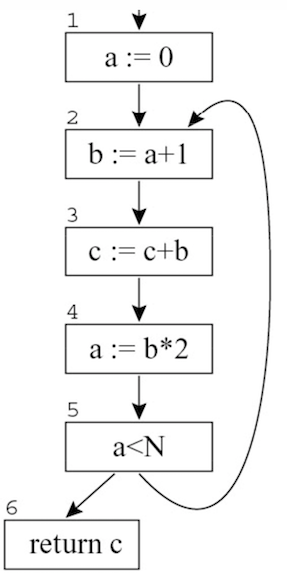
\includegraphics[scale=0.75]{image/reachingDefExam}
	\caption{Một đoạn chương trình mẫu}
	\label{fig:reachingdefexam}
\end{figure}
Ví dụ như ở đoạn chương trình \ref{fig:reachingdefexam}, cần biết được giá trị của biến \textit{a} ở câu lệnh số 2 được khai báo ở câu lệnh nào. Đối với con người thì rất dễ dàng biết được là biến \textit{a} được sử dụng có thể khai báo ở câu lệnh số 1 hoặc câu lệnh số 5. Tuy nhiên, cần có một phương pháp phân tích để cho máy tính cũng biết được điều đó, và đó chính là phương pháp Reaching definitions. Như vậy, khi áp dụng vào trình dịch ngược, ta sẽ biết được tại thời điểm sử dụng biến bit, giá trị của thanh ghi \textit{ACC} đang được định nghĩa ở câu lệnh nào. Từ đó tiến hành các bước kiểm tra tiếp theo. \\

Để thực hiện Reaching definitions, ta phải làm quen với các định nghĩa sau:
\begin{itemize}
	\item Nếu một biến được khai báo ở câu lệnh \textit{def1}, sau đó được khai báo lại ở câu lệnh \textit{def2} sau đó, thì ta nói là câu lệnh \textit{def1} đã \textbf{bị giết (killed)} bởi câu lệnh \textit{def2}.
	\item Nếu có một đường thực thi chương trình đi từ câu lệnh khai báo \textit{def1} đến một điểm \textit{p} của chương trình, mà trên đó \textit{def1} không bị giết bởi bất kỳ câu lệnh nào, thì ta nói là \textit{def1} đã \textbf{đến được (reach))} điểm \textit{p}. Khái niệm một câu lệnh đến được một khối cơ bản cũng tương tự như vậy.
\end{itemize}

Ngoài ra, ta phải quy định một số khái niệm mới cho một khối cơ bản B:
\begin{itemize}
	\item \textit{REACHin(B)}: Tập hợp các câu lệnh khai báo đến được đầu vào (entry) của B.
	\item \textit{REACHout(B)}: Tập hợp các câu lệnh khai báo đến được ngõ ra (exit) của B.
	\item \textit{GEN(B)}: Tập hợp các câu lệnh khai báo xuất hiện trong B và có thể đến được ngõ ra (exit) của B, nghĩa là biến được khai báo trong câu lệnh đó không được khai báo lại ở các câu lệnh đằng sau nó.
	\item \textit{KILL(B)}: Tập hợp các câu lệnh khai báo mà biến được khai báo đã được khai báo lại trong B.
\end{itemize}

Như vậy, mục tiêu của phân tích Reaching definitions ở cấp độ khối cơ bản là tìm ra được tập hợp \textit{REACHin} và \textit{REACHout} của từng khối. Công thức được áp dụng là;
\begin{equation} \label{eq:reachout}
	REACHout(B) = GEN(B) \cup (REACHin(B)-KILL(B))
\end{equation}	
\begin{equation} \label{eq:reachin}
REACHin(B) = \cup_{j \in Pred(B)} REACHout(j)
\end{equation}	

Từ hai công thức \ref{eq:reachout} và \ref{eq:reachin}, ta thấy ở phân tích này, tập hợp các giá trị ra (\textit{REACHin}) được quyết định bởi các giá trị vào (\textit{REACHout}), ngược lại với phân tích liveness (tìm tập hợp biến đang sống tại một thời điểm của chương trình). Như vậy, luồng đi của phân tích là cùng chiều với luồng đi của chương trình. Tương tự một số phương pháp phân tích dữ liệu khác, ta sẽ lần lượt tính toán các tập hợp vào và tập hợp ra của từng khối cơ bản cho đến khi không còn thay đổi nào được ghi nhận. Xem sơ đồ khối hình \ref{fig:reachingdefalgo}.



Tuy nhiên, trong trường hợp của bài toán cần giải quyết, ta cần phải biết tập hợp ra vào của từng câu lệnh một, chứ không chỉ của toàn bộ khối cơ bản, vì vậy, khi ứng dụng vào Boomerang, giải thuật sẽ được điều chỉnh lại để tìm tập \textit{REACHin} và \textit{REACHout} của từng câu lệnh. Việc điều chỉnh này là khá nhỏ, và các bước vẫn sẽ giữ nguyên, không thay đổi nhiều.\\

Khuyết điểm lớn nhất của phân tích Reaching definitions chỉ cho biết được câu lệnh khai báo có hiệu lực của một biến tại một thời điểm chương trình, chứ không cho biết được giá trị thực sự của biến đó. Cụ thể, với thanh ghi \textit{ACC}, nếu vế phải của câu lệnh khai báo này chỉ đơn giản là trỏ đến một vùng nhớ có địa chỉ được quy định bởi một biến byte thì biến byte đó sẽ được ghi nhận là đại diện cho vùng nhớ hiện thời \textit{ACC} đang lưu trữ. Nhưng ngoài ra, biểu thức quy định địa chỉ vùng nhớ được gán cho \textit{ACC} có thể là các trường hợp sau đây:
\begin{itemize}
	\item Một hằng số.
		\item Một thanh ghi, giá trị của thanh ghi có thể được khai báo ở các câu lệnh trước đó.
	\item Một biểu thức có hai vế, các vế của biểu thức có thể là một biến, một thanh ghi hoặc một hằng số.

\end{itemize}

\begin{lstlisting}[caption={Một số câu lệnh gán mà phương pháp Suy luận kiểu sử dụng Reaching definitions không xử lý được},label={list:listhardcase}]
MOV A, 38H #1
MOV A, @DPTR #2
MOV A, OPTION+1 #3
\end{lstlisting}
Các trường hợp phức tạp nêu trên được trình bày trong đoạn mã \ref{list:listhardcase}. 
Phương pháp Reaching definitions sẽ không thể xử lý được khi gặp các câu lệnh gán này. Ở câu lệnh số 1, phân tích có thể lấy được giá trị \textbf{38H}, nhưng không thể xác định được biến byte nào đã được khai báo giá trị \textbf{38H}. Ở câu lệnh số 2, Reaching definitions không thể biết được giá trị của thanh ghi \textit{DPTR} là bao nhiêu. Ở câu lệnh số 3, việc xử lý lại càng phức tạp hơn, vì nếu chỉ đơn giản lấy vế phải của khai báo ra, không thể nào biết được giá trị thực sự của nó là bao nhiêu.
Ngoài ra, với trường hợp trong tập hợp \textit{REACHin} của câu lệnh có nhiều câu lệnh khai báo cho thanh ghi \textit{ACC}, phương pháp này sẽ không thể kiểm tra được vế phải của tất cả các câu lệnh khai báo đó có cùng một giá trị hay không mà chỉ đơn giản xử lý là câu lệnh đã vi phạm nguyên tắc sử dụng bộ biến. Ví dụ như đoạn mã \ref{list:ifcond}, tại thời điểm câu lệnh sử dụng biến bit \textit{TESTSUPS}, có hai câu lệnh khai báo biến \textit{a} (là biến đại diện cho thanh ghi \textit{ACC} tại ngôn ngữ trung gian). Đối với phương pháp Reaching definitions, nó sẽ xem như có hai giá trị mà biến \textit{a} có thể mang, và sẽ báo lỗi vì vi phạm nguyên tắc sử dụng bộ biến. Tuy nhiên, nếu xét kỹ hơn, thì sẽ thấy là cả hai giá trị đó đều là biến \textit{OPTIONS}, và thực chất tại thời điểm này \textit{a} chỉ mang một giá trị, cho dù luồng đi của chương trình có như thế nào. Như vậy, phương pháp Reaching definitions sẽ bỏ qua những trường hợp như thế này và báo lỗi, dẫn đến việc độ chính xác sẽ không được cao.
\begin{lstlisting}[caption={Đoạn mã có nhiều câu lệnh khai báo cho ACC đến được một điểm của chương trình nhưng tất cả đều cùng giá trị},label={list:ifcond}]
if (...){
	a = *(OPTIONS);
	...
} else {
	a = *(OPTIONS);
	...
}
TESTSUPS = 1;
\end{lstlisting}

Để khắc phục phần nào khuyết điểm của Reaching definitions, một phần mở rộng được thêm vào để giải quyết một trong những trường hợp mà phương pháp này không thể giải quyết được. Đó là trường hợp sử dụng một biến trung gian và sử dụng hằng (câu lệnh số 1 và số 2 ở đoạn mã \ref{list:listhardcase}). Các trường hợp này được giải quyết nhờ vào việc lưu trữ các khai báo \textit{\#DEFINE} ở đoạn mã đầu vào, cũng như trong quá trình phân tích, tất cả các câu lệnh khai báo của tất cả các biến đến được một điểm trong chương trình đều được lưu giữ chứ không chỉ riêng của thanh ghi \textit{ACC}. Cụ thể các bước của phần mở rộng được trình bày ở hình \ref{fig:reachdefextendalgo}.
\begin{figure}
	\centering
	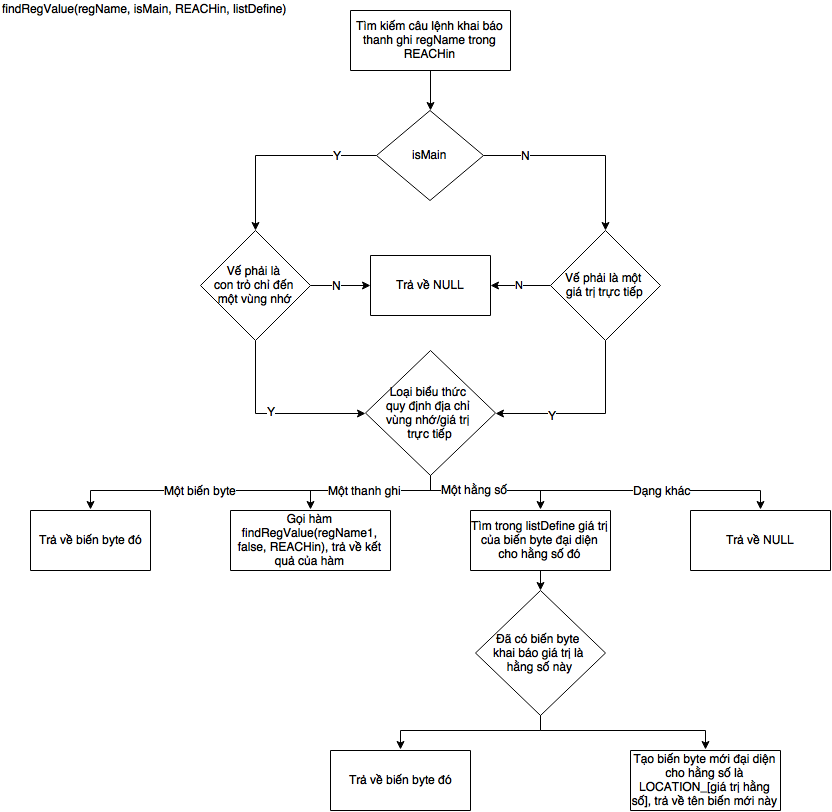
\includegraphics[width=0.7\linewidth]{image/reachdefextendalgo}
	\caption{Giải thuật cho hàm findRegValue - phần mở rộng của phân tích Reaching definitions}
	\label{fig:reachdefextendalgo}
\end{figure}

Theo giải thuật nêu trên, để tìm được giá trị của thanh ghi \textit{ACC} tại một thời điểm của chương trình, cần truyền vào hàm \textit{findRegValue} tên thanh ghi ("ACC"), giá trị true để hàm biết đang tìm kiếm giá trị cho thanh ghi \textit{ACC}, tập \textit{REACHin} tại thời điểm đó của chương trình và danh sách các cặp tên biến - giá trị biến được khai báo ở phần đầu của mã đầu vào. Qua các bước của giải thuật, hàm sẽ trả về giá trị là biến byte quy định vùng nhớ được load dữ liệu vào \textit{ACC} nếu tìm được biến này, còn nếu trả về giá trị \textbf{NULL}, nghĩa là giải thuật đã gặp phải trường hợp không xử lý được, đó là trường hợp biểu thức vế phải gồm hai toán hạng (câu lệnh số 3 của đoạn mã \ref{list:listhardcase}).

Tuy đã xử lý được hầu hết các trường hợp của phép gán cho \textit{ACC}, nhưng việc có thêm một phần mở rộng này sẽ làm cho tốc độ xử lý trình dịch ngược giảm đi. Cộng thêm việc bản thân giải thuật Reaching definitions đã có độ phức tạp cao, tổng thời gian xử lý cho bước này của trình dịch ngược là khá lớn. Vì vậy, một phương pháp phân tích khác đã được thực hiện để tìm ra giá trị của thanh ghi \textit{ACC} với độ phức tạp thấp hơn.

\subsubsection{Phân tích Type propagation}
Phân tích Type propagation có mục đích sẽ tìm ra được kiểu của một thanh ghi bằng cách lan truyền kiểu của những thanh ghi khác. Áp dụng vào trường hợp cụ thể của luận văn, các tên biến byte có thể được xem là một kiểu, vì khi chuyển đổi bộ biến thành một kiểu union ở ngôn ngữ cấp cao, tên biến byte này sẽ được dùng để đặt tên cho kiểu union đó. Như vậy, tác dụng của phân tích Type propagation này là tìm ra được thanh ghi \textit{ACC} đang mang kiểu union nào tại một thời điểm của chương trình. Các bước của giải thuật phân tích Type propagation được trình bày ở hình \ref{fig:typepropagationalgo}.

\begin{figure}[h!]
	\centering
	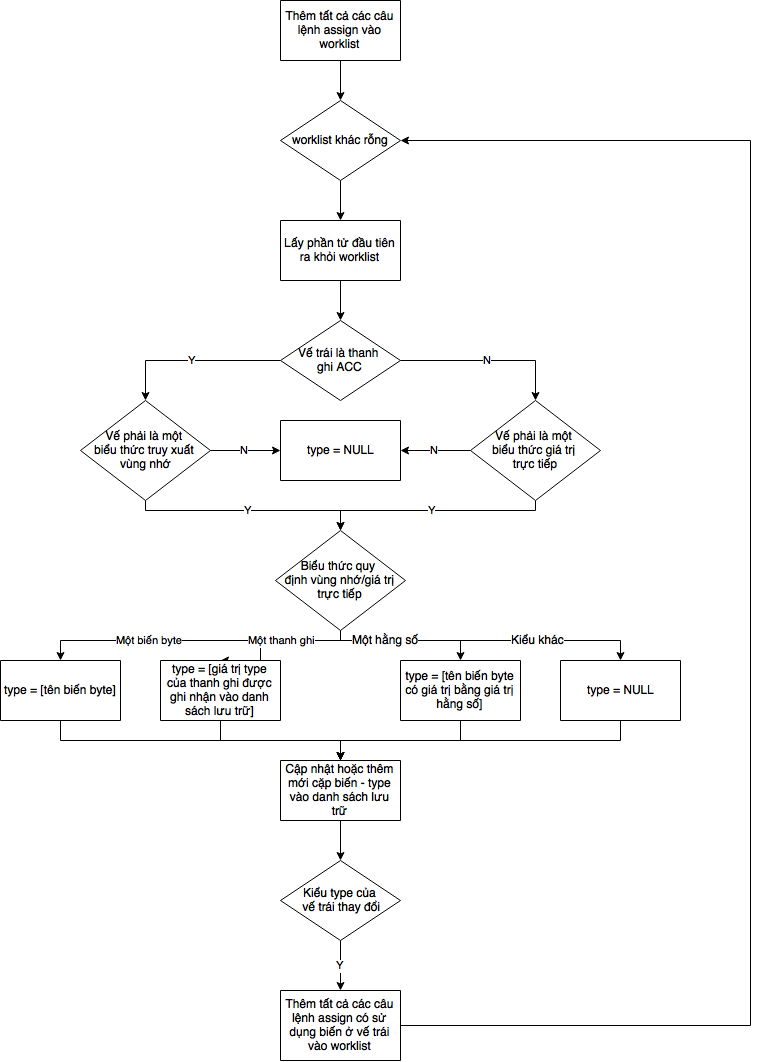
\includegraphics[width=0.7\linewidth]{image/typePropagationAlgo}
	\caption{Giải thuật của phân tích Type propagation}
	\label{fig:typepropagationalgo}
\end{figure}

Trong giải thuật đã trình bày ở trên, không xét đến trường hợp một biến được khai báo lại nhiều lần và tại mỗi thời điểm sẽ có giá trị khác nhau là do tận dụng được mã trung gian \textit{SSA}. Hầu hết các trình dịch ngược đều sử dụng mã \textit{SSA} tại một giai đoạn nào đó trong quá trình phân tích dữ liệu vì các lợi ích của loại mã này (chi tiết về mã \textit{SSA} được trình bày trong phần \ref{ssa}). Với mã \textit{SSA}, mỗi biến chỉ được khai báo một lần duy nhất trong chương trình, nên không bị ảnh hưởng bởi trường hợp khai báo lại biến.\\

Như vậy, phương pháp Type propagation này sẽ làm giảm đáng kể thời gian xử lý của chương trình so với phương pháp Reaching definitions. Khi có một thay đổi nào đó, chương trình phân tích chỉ cần tính toán lại các câu lệnh khai báo chịu ảnh hưởng của sự thay đổi đó, chứ không cần phải tính toán lại hết tất cả các câu lệnh như giải thuật của Reaching definitions. Phương pháp này cũng không cần một phần mở rộng mà ngay trong quá trình lan truyền, nó đã tính toán được các trường hợp biểu thức vế phải của khai báo là một thanh ghi hoặc một hằng số. Khuyết điểm của Type propagation là vẫn chưa xử lý được trường hợp biểu thức vế phải có hai toán hạng. Để giải quyết được vấn đề này, cần có một phân tích khác mạnh hơn và phân tích đó sẽ được giới thiệu ở chương tiếp theo.
\subsection{Kiểm tra tính hợp lệ về kiểu của tác vụ với bit}

\label{sec:laststep}

Sau khi đã tìm được thông tin về kiểu của thanh ghi \textit{ACC} tại mỗi điểm của chương trình, bước tiếp theo của giải pháp Kiểm tra kiểu là kiểm tra tính hợp lệ khi sử dụng các biến bit. Như đã trình bày ở phần \ref{sec:problem}, việc sử dụng các \textbf{biến byte - biến bit} trong mã chương trình 8051 cần tuân thủ các quy định sau:
\begin{itemize}
	\item Chỉ khi thanh ghi \textit{ACC} đang mang giá trị của vùng nhớ có địa chỉ quy định bởi biến byte, thì các biến bit cùng bộ mới được sử dụng.
	\item Mỗi biến bit chỉ thuộc một bộ duy nhất. 
	\item Tại mỗi vị trí bit của một bộ biến chỉ có một biến bit duy nhất tồn tại. 
\end{itemize}
Như vậy, ở phần này, chương trình sẽ chạy vòng lặp kiểm tra lần lượt từng câu lệnh sử dụng bit để xem xét việc sử dụng này có vi phạm quy định nào trong những quy định trên hay không. Các bước kiểm tra này được trình bày ở hình \ref{fig:checkunionsteps}.
\begin{figure}
	\centering
	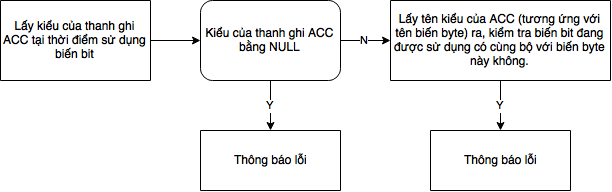
\includegraphics[width=0.7\linewidth]{image/checkUnionSteps}
	\caption{Quá trình kiểm tra một câu lệnh sử dụng bit}
	\label{fig:checkunionsteps}
\end{figure}
Nếu có một câu lệnh sử dụng bit nào đó vi phạm nguyên tắc trên, chương trình kiểm tra vẫn tiếp tục chạy để kiểm tra những câu lệnh sau đó. Điều này giúp người lập trình biết được tất cả các lỗi trong chương trình đầu vào của mình để có sự chỉnh sửa phù hợp. Tuy nhiên, khi có vi phạm xảy ra, trình dịch ngược sẽ không sinh được mã đầu ra, vì không có cách thể hiện union phù hợp.

%đoạn mã và output của trình dịch ngược khi vi phạm nguyên tắc sử dụng

Như vậy, với giải pháp Kiểm tra kiểu, ta đã có sẵn thông tin về bộ biến ngay từ đầu và chỉ cần kiểm tra xem người lập trình có tuân thủ đúng quy tắc không trước khi sinh ra mã ở ngôn ngữ cấp cao. Giải pháp này yêu cầu can thiệp vào trình dịch ngược ít và hiện thực dễ dàng. Tuy nhiên, giải pháp còn nhiều hạn chế như phương pháp phân tích dữ liệu chưa đạt độ chính xác cao, cần người dùng phải chỉnh sửa lại chú thích theo mẫu quy định... Chính vì vậy, giai đoạn sau của luận văn đã phát triển một hướng tiếp cận mới có độ chính xác cao hơn và không cần chỉnh sửa mã đầu vào của người dùng, đó là giải pháp Suy luận kiểu. Giải pháp này sẽ được trình bày ở chương tiếp theo.



